\documentclass[aps,prd,onecolumn,nofootinbib,superscriptaddress]{revtex4-2}

% ----------------------------------------
% Packages
% ----------------------------------------
\usepackage[utf8]{inputenc}
\usepackage[T1]{fontenc}
\usepackage{lmodern}
\usepackage{amsmath,amssymb,amsfonts,bm}
\usepackage{graphicx}
\usepackage{xcolor}
\usepackage{hyperref}
\usepackage{siunitx}
\usepackage{enumitem}

\hypersetup{
  colorlinks=true,
  linkcolor=blue,
  citecolor=blue,
  urlcolor=blue
}

% ----------------------------------------
% Shortcuts
% ----------------------------------------
\newcommand{\Mpl}{M_{\rm Pl}}
\newcommand{\Meff}{M_{\rm eff}}
\newcommand{\Om}{\Omega}
\newcommand{\Omb}{\Omega_{\rm b}}
\newcommand{\Omc}{\Omega_{\rm c}}
\newcommand{\Omm}{\Omega_{\rm m}}
\newcommand{\Oml}{\Omega_{\Lambda}}
\newcommand{\Omg}{\Omega_{\gamma}}
\newcommand{\Omr}{\Omega_{\rm r}}
\newcommand{\Hinf}{H_{\rm inf}}
\newcommand{\As}{A_{\rm s}}
\newcommand{\ns}{n_{\rm s}}
\newcommand{\trm}{\mathrm}
\newcommand{\dd}{\mathrm{d}}

\begin{document}

% ----------------------------------------
% Title and abstract
% ----------------------------------------

\title{TCV-$\phi$ I: an effective cohesive--vacuum field theory \\
and its $\Lambda$CDM--compatible background cosmology}

\author{Cyrille LECROQ}
\affiliation{Independant Researcher}

\date{2025}

\begin{abstract}
We introduce the first step of the ``TCV-$\phi$'' programme, in which the late--time cosmological expansion and cold dark matter are reinterpreted in terms of a cohesive vacuum carrying two scalar degrees of freedom.
At the effective field theory (EFT) level, we consider a minimal scalar--tensor model with a ``structural'' scalar field $\Phi_1$ and a light coherent field $\Phi_2$, coupled to gravity via a slightly non--minimal Planck mass $\Meff^2(\Phi_1)$ and a simple cohesive potential $V(\Phi_1,\Phi_2)$.
In this first paper we focus deliberately on the homogeneous background and linear matter power spectrum.
We show that: (i) for a reasonable benchmark set of microscopic parameters, the background expansion history $H(z)$ can be made practically indistinguishable from vanilla $\Lambda$CDM, with parameter values close to Planck 2018; (ii) the coherent field $\Phi_2$ naturally behaves as an ultra--light dark matter (ULDM) component once $H\ll m_2$, with energy density scaling as $a^{-3}$; (iii) by interfacing the TCV-$\phi$ EFT with the Boltzmann code CLASS and by applying a simple fuzzy--DM transfer function, we obtain a matter power spectrum $P(k)$ whose large--scale behaviour is $\Lambda$CDM--like and whose small--scale suppression is of the type usually associated with ULDM.
Crucially, in this first paper we do not attempt to derive all cosmological parameters from the microphysics: the scalar masses, self--couplings and the initial misalignment of $\Phi_2$ are treated as phenomenological EFT parameters, chosen to be close to current best--fit $\Lambda$CDM values. Our only requirement is that the illustrative ULDM--like suppression leaves the large--scale spectrum essentially unchanged; a full quantitative confrontation with CMB and large--scale structure data is postponed to future work.
\end{abstract}

\maketitle

% ----------------------------------------
\section{Introduction}
% ----------------------------------------

The standard cosmological model, $\Lambda$CDM with slow--roll inflation and cold dark matter, provides an excellent fit to most available data, from the cosmic microwave background (CMB) anisotropies to large--scale structure (LSS) and baryon acoustic oscillations (BAO).
At the same time, it leaves several conceptual questions open:
What is the microscopic origin of the cosmological constant?
Why does dark matter appear cold and collisionless on large scales, yet possibly cored or suppressed on the smallest observable scales?
Can one relate early-- and late--time physics within a single effective framework, rather than with a collection of loosely connected sectors?

The ``TCV-$\phi$'' (for ``Théorie du Vide Cohésif'') programme is an attempt to address these questions within a simple scalar--tensor EFT, in which the gravitational sector is supplemented by two real scalar fields:
\begin{itemize}[leftmargin=1.5em]
  \item a \emph{structural} field $\Phi_1$, responsible for encoding the cohesive properties of the vacuum and a mild non--minimal coupling to gravity;
  \item a light \emph{coherent} field $\Phi_2$, behaving at late times as an ultra--light dark matter (ULDM) component.
\end{itemize}
At the purely phenomenological level, the TCV-$\phi$ EFT can be tuned to reproduce standard $\Lambda$CDM background cosmology plus ULDM--like suppression of small--scale power, while from a conceptual point of view it provides a single Lagrangian from which we intend to derive, in later papers, a bounce cosmology, spontaneous baryogenesis, and regular black holes with cohesive cores.

In this first paper, our goals are intentionally modest and conservative:
\begin{enumerate}[label=(\roman*),leftmargin=1.5em]
  \item to define clearly the effective field content and potential of the TCV-$\phi$ model;
  \item to show how, at the homogeneous level, this EFT reproduces a $\Lambda$CDM--like expansion history for a benchmark choice of parameters;
  \item to interface the EFT with the Boltzmann code CLASS and to illustrate how a simple fuzzy--DM transfer function acting on the cold dark matter power spectrum leads to an \emph{illustrative} matter power spectrum $P(k)$ that coincides with $\Lambda$CDM on large scales while exhibiting an ULDM--like suppression on small scales, without attempting a quantitative comparison to data in this paper;
  \item to keep track of, and explicitly label, which quantities are \emph{assumed} phenomenological parameters at this stage (masses, couplings, misalignment amplitudes), and which ones are \emph{derived} from them at the cosmological level.
\end{enumerate}

It is important to emphasize that this first paper does not aim at introducing genuinely new cosmological phenomenology beyond standard $\Lambda$CDM plus an ultralight dark-matter component. Rather, our goal is to define a minimal cohesive--vacuum EFT, to check that it admits a healthy $\Lambda$CDM-like background and a plausible ULDM sector, and to provide a transparent baseline that will be used in subsequent TCV-$\phi$ papers on the bounce, baryogenesis and black holes.

Our construction is therefore close in spirit to existing models where gravity is minimally or non-minimally coupled to one or more scalar fields, with one heavy field stabilized at late times and a light ultralight component playing the role of dark matter. Examples include scalar--tensor theories with stabilized moduli (see e.g.\ the review~\cite{Clifton2012}), quintessence + axion models and the extensive literature on fuzzy or ultralight dark matter~\cite{ULDM,Hui2017,Marsh2016,Schive2014}. What is specific to the TCV-$\phi$ programme is not the late-time cosmological phenomenology explored here, but the fact that the same EFT will be used, in later work, to describe a cohesive bounce, spontaneous baryogenesis and regular black holes with cohesive cores within a unified Lagrangian framework.

Throughout the paper we work in units $c=\hbar=1$ and adopt a reduced Planck mass $\Mpl \simeq 2.435\times 10^{18}\,\mathrm{GeV}$.
We follow the usual convention for cosmological parameters $H_0=100\,h\,\mathrm{km\,s^{-1}\,Mpc^{-1}}$, $\Omega_i$ and $\omega_i\equiv\Omega_i h^2$.

% ----------------------------------------
\section{Cohesive--vacuum EFT: fields and potential}
\label{sec:EFT}
% ----------------------------------------

\subsection{Action and non--minimal coupling}

At the EFT level, the TCV-$\phi$ model is defined by the following action:
\begin{align}
  S &= \int \dd^4x\,\sqrt{-g}
  \Bigg[
    \frac{1}{2}\Meff^2(\Phi_1) R
    - \frac{1}{2}(\nabla\Phi_1)^2
    - \frac{1}{2}(\nabla\Phi_2)^2
    - V(\Phi_1,\Phi_2)
  \Bigg]
  + S_{\rm SM}[g_{\mu\nu},\Psi_{\rm SM}],
  \label{eq:action}
\end{align}
where $R$ is the Ricci scalar, $\Meff^2(\Phi_1)$ is an effective (field-dependent) Planck mass, $V(\Phi_1,\Phi_2)$ is the cohesive potential, and $S_{\rm SM}$ encodes the Standard Model and baryonic matter.

In the present paper we adopt a simple non--minimal coupling of the form
\begin{align}
  \Meff^2(\Phi_1)
  &=
  \Mpl^2\left( 1 + \xi_0 \frac{\Phi_1^2}{\Mpl^2} \right),
  \label{eq:Meff}
\end{align}
with a small dimensionless constant $\xi_0$.
For the purposes of the present paper we work in a regime where the variation of $\Meff^2$ around its late-time value is completely negligible. Around the minimum $\Phi_1 \simeq \Phi_0$ we have
\begin{equation}
  \frac{\Delta \Meff^2}{\Meff^2}
  \simeq \xi_0\,\frac{\Phi_1^2 - \Phi_0^2}{\Mpl^2}
  \lesssim \xi_0\,\frac{\Phi_0^2}{\Mpl^2}.
\end{equation}
With our benchmark values $m_1 \sim \Phi_0 \sim 10^{11}\,\mathrm{GeV}$ and $\xi_0 \sim 0.1$, this gives
\begin{equation}
  \left|\frac{\Delta \Meff^2}{\Meff^2}\right|
  \lesssim \xi_0 \left(\frac{\Phi_0}{\Mpl}\right)^2
  \sim 0.1 \times \left(\frac{10^{11}}{2.4\times 10^{18}}\right)^2
  \sim 10^{-16},
\end{equation}
many orders of magnitude below current bounds on the variation of Newton's constant from BBN, CMB and local tests of gravity. In addition, the time derivatives $\dot \Meff$ and $\ddot \Meff$ in the background equations are suppressed by the large mass scale $m_1$ compared to the Hubble rate $H$. It is therefore self-consistent, for the late-time homogeneous cosmology considered here, to neglect the non-minimal terms and to use GR-like Friedmann and Klein--Gordon equations with a nearly constant Planck mass. A more explicit estimate of the variation of $M_{\rm eff}$ and of the associated bounds from constraints on the variation of Newton's constant is given in Appendix~\ref{app:Meff}.
For the background cosmology and the mildly perturbed regimes considered in Paper~I, the variation of $\Meff^2$ around its present value is negligible, so that one can think of
\begin{equation}
  \Meff^2(\Phi_1) \simeq \Mpl^2
\end{equation}
as a very good approximation at late times.
Nevertheless we keep track of the dependence on $\Phi_1$ because it plays a central role in later TCV-$\phi$ work (bounce dynamics and black holes).

\subsection{Cohesive potential}

We choose a potential separable in the two scalars:
\begin{equation}
  V(\Phi_1,\Phi_2) = V_1(\Phi_1) + V_2(\Phi_2) + \rho_{\rm vac},
\end{equation}
with
\begin{align}
  V_1(\Phi_1)
  &= \frac{1}{2}m_1^2 (\Phi_1 - \Phi_0)^2
   + \frac{\lambda_1}{4} (\Phi_1 - \Phi_0)^4,
  \label{eq:V1-def}
  \\
  V_2(\Phi_2)
  &= \frac{1}{2}m_2^2 \Phi_2^2,
  \label{eq:V2-def}
\end{align}
and a small vacuum offset $\rho_{\rm vac}$, chosen such that the effective cosmological constant today matches the observed dark energy density.

The microscopic parameters of the EFT are then
\begin{equation}
  \{m_1,\,\Phi_0,\,\lambda_1,\,\xi_0,\,m_2,\,\rho_{\rm vac},\,\Mpl\}.
\end{equation}
In subsequent papers, an additional cubic self--interaction $\kappa(\Phi_1-\Phi_0)^3$ and a baryogenesis scale $\Lambda_B$ are introduced; for the background cosmology of Paper~I these extra parameters do not play a role and we omit them here for clarity.

The potential~\eqref{eq:V1-def} is minimized at $\Phi_1=\Phi_0$, with curvature
\begin{equation}
  m_{\rm eff,1}^2 \equiv \left.\frac{\partial^2 V_1}{\partial\Phi_1^2}\right|_{\Phi_1=\Phi_0}
  = m_1^2,
\end{equation}
and we typically choose $m_1\sim \Phi_0\sim 10^{11}\,\mathrm{GeV}$ as a benchmark, so that the structural field is extremely heavy compared to any cosmological scale.
We have checked numerically, with the test scripts shipped in the \texttt{TCV-Phi} repository, that for this potential
\begin{equation}
  V_1(\Phi_0) = 0,\qquad
  \partial_{\Phi_1} V_1(\Phi_0)=0,\qquad
  \partial^2_{\Phi_1} V_1(\Phi_0) = m_1^2 >0,
\end{equation}
so that $\Phi_1$ sits in a stable minimum at late times.

The potential $V_2(\Phi_2)$ is that of a standard ULDM--like scalar:
we take
\begin{equation}
  m_2 \simeq 10^{-22}\,\mathrm{eV}
  \quad \Longleftrightarrow \quad
  m_2 \simeq 10^{-31}\,\mathrm{GeV},
\end{equation}
and we assume that $\Phi_2$ starts with some misalignment amplitude $\Phi_{2,0}$ in the early universe, such that its coherent oscillations reproduce the observed dark matter abundance today.
At this stage $\Phi_{2,0}$ is treated as a phenomenological parameter fixed by the requirement $\Omega_{\rm dm} h^2\simeq 0.12$; we will comment on this in more detail below.

% ----------------------------------------
\section{Background cosmology and effective $\Lambda$CDM mapping}
\label{sec:background}
% ----------------------------------------

\subsection{Homogeneous equations}

We consider a spatially flat Friedmann--Lemaître--Robertson--Walker (FLRW) background,
\begin{equation}
  \dd s^2 = -\dd t^2 + a^2(t)\,\dd\vec{x}^2,
\end{equation}
with homogeneous scalar fields $\Phi_1(t)$ and $\Phi_2(t)$.
The modified Friedmann equations derived from~\eqref{eq:action} can be written, in the regime where $\Meff^2(\Phi_1)\simeq\Mpl^2$ is slowly varying, as
\begin{align}
  3\Mpl^2 H^2
  &= \rho_{\rm SM} + \rho_{\Phi_1} + \rho_{\Phi_2} + \rho_{\rm vac},
  \label{eq:Friedmann1}
  \\
  -2\Mpl^2 \dot H
  &= \rho_{\rm SM}+p_{\rm SM} + \dot\Phi_1^2 + \dot\Phi_2^2,
  \label{eq:Friedmann2}
\end{align}
with
\begin{align}
  \rho_{\Phi_1}
  &= \frac12 \dot\Phi_1^2 + V_1(\Phi_1),
  &
  p_{\Phi_1}
  &= \frac12 \dot\Phi_1^2 - V_1(\Phi_1),
  \\
  \rho_{\Phi_2}
  &= \frac12 \dot\Phi_2^2 + V_2(\Phi_2),
  &
  p_{\Phi_2}
  &= \frac12 \dot\Phi_2^2 - V_2(\Phi_2).
\end{align}
The Klein--Gordon equations for the homogeneous modes read
\begin{align}
  \ddot\Phi_1 + 3H\dot\Phi_1 + \frac{\partial V_1}{\partial\Phi_1}
  &\simeq 0,
  \label{eq:KG1}
  \\
  \ddot\Phi_2 + 3H\dot\Phi_2 + m_2^2 \Phi_2
  &= 0.
  \label{eq:KG2}
\end{align}
In~\eqref{eq:KG1}, we have neglected the small contributions coming from the non--minimal coupling, which are suppressed by the large mass scale $\Mpl/\xi_0$ and irrelevant for the late--time homogeneous cosmology of interest here.

\subsection{Late--time regime and ULDM behaviour}

Around the minimum $\Phi_1\simeq \Phi_0$ the structural field is extremely heavy,
\begin{equation}
  m_1 \gg H(t)
\end{equation}
for all cosmological times after reheating.
As a result, $\Phi_1$ relaxes very quickly towards its minimum and remains essentially frozen, $\Phi_1(t)\simeq \Phi_0$, with negligible kinetic energy.
Its main effect on the homogeneous background, in the present paper, is therefore to provide a nearly constant vacuum contribution $\rho_{\rm vac}$ that we identify with the observed dark energy density,
\begin{equation}
  \rho_\Lambda^{\rm eff} = \rho_{\rm vac} 
  \simeq (2.26\times 10^{-3}\,\mathrm{eV})^4.
\end{equation}
A more detailed discussion of how $\rho_{\rm vac}$ arises from the cohesive microphysics is postponed to later TCV-$\phi$ work.

The light scalar $\Phi_2$ behaves as standard ULDM when $H\ll m_2$:
the solution of~\eqref{eq:KG2} in this regime is well approximated by
\begin{equation}
  \Phi_2(t) \simeq \Phi_{2,0}\,a^{-3/2}(t)\cos(m_2 t+\delta),
\end{equation}
with slowly varying amplitude and phase.
Averaging over many oscillations, the effective energy density scales as
\begin{equation}
  \bar\rho_{\Phi_2} \propto a^{-3},
\end{equation}
so that $\Phi_2$ behaves as pressureless matter at the background level.
Using the standard misalignment estimate for ULDM, one finds that the relic density today is approximately
\begin{equation}
  \Omega_{\Phi_2} h^2
  \simeq 0.1\,
  \left(\frac{\Phi_{2,0}}{10^{17}~\mathrm{GeV}}\right)^2
  \left(\frac{m_2}{10^{-22}~\mathrm{eV}}\right)^{1/2},
  \label{eq:misalignment}
\end{equation}
This is the standard order-of-magnitude misalignment estimate for ultralight scalar dark matter (see e.g.\ Refs.~\cite{ULDM,Hui2017,Marsh2016}); the numerical prefactor depends only mildly on the precise onset of oscillations and on the thermal history. In this paper we use Eq.~\eqref{eq:misalignment} as a phenomenological mapping between $(m_2,\Phi_{2,0})$ and $\Omega_{\Phi_2} h^2$, rather than as a precision calculation.
In the TCV-$\phi$ benchmark used in our numerical tests, we choose
\begin{equation}
  m_2 \simeq 10^{-22}~\mathrm{eV},\qquad
  \Phi_{2,0} \simeq 1.1\times 10^{17}~\mathrm{GeV},
\end{equation}
In terms of the reduced Planck mass, this corresponds to $\Phi_{2,0} / \Mpl \simeq 0.05$, i.e.\ a sub-Planckian field excursion that remains within the usual EFT regime.
which gives
\begin{equation}
  \Omega_{\Phi_2} h^2 \simeq 0.12,
\end{equation}
so that the coherent field $\Phi_2$ accounts for essentially the entire dark matter abundance.
At this stage we treat~\eqref{eq:misalignment} as a phenomenological mapping between EFT parameters and cosmological ones; we do not yet attempt to derive $\Phi_{2,0}$ from the cohesive microphysics of $\Phi_1$.

\subsection{Effective $\Lambda$CDM parameter set}

Summarising, at the homogeneous level the TCV-$\phi$ EFT provides:
\begin{itemize}[leftmargin=1.5em]
  \item a dark energy component with energy density $\rho_\Lambda^{\rm eff}=\rho_{\rm vac}$,
  \item a dark matter component with energy density $\rho_{\rm dm}=\bar\rho_{\Phi_2}$,
  \item standard baryons and radiation provided by the Standard Model sector.
\end{itemize}
The effective cosmological parameter set that we feed to CLASS in this first paper is therefore
\begin{align}
  H_0 &= 67.4~\mathrm{km\,s^{-1}\,Mpc^{-1}},
  &
  \omega_{\rm b} &= \Omega_{\rm b} h^2 \simeq 0.0224,
  &
  \omega_{\rm c} &= \Omega_{\rm dm} h^2 \simeq 0.12,
  \nonumber\\
  \omega_\gamma &= 2.47\times 10^{-5},
  &
  \omega_\nu &\simeq 1.7\times 10^{-5},
  &
  \Omega_\Lambda^{\rm eff} &= 1 - \Omega_{\rm m} - \Omega_{\rm r},
  \label{eq:theta-tcv}
\end{align}
with $\Omega_{\rm m}=\Omb+\Omc$ and $\Omega_{\rm r}=\Omg+\Omega_\nu$.
Our reference benchmark is chosen to be close to the Planck 2018 best--fit cosmology.
We have implemented a small Python module (distributed in the \texttt{TCV-Phi} repository) that builds a dictionary of TCV--$\phi$--compatible CLASS inputs, and a test script \texttt{test\_tcv\_background.py} that prints the associated $\Omega_i$ and the background evolution.

For the benchmark above, we find numerically
\begin{align}
  \Omb &\simeq 0.0493,
  &
  \Omc &\simeq 0.2642,
  &
  \Omm &\simeq 0.3135,
  \\
  \Omr &\simeq 9\times 10^{-5},
  &
  \Oml &\simeq 0.6864,
\end{align}
so that the background expansion history is essentially indistinguishable from vanilla $\Lambda$CDM at the current level of precision.
In the context of this first paper, the TCV-$\phi$ model should therefore be viewed as a \emph{reinterpretation} of a standard $\Lambda$CDM background in terms of a cohesive vacuum and a coherent ULDM field, rather than as a modification of the homogeneous cosmology.

To make this statement more quantitative, we compare the TCV-$\phi$
background to a reference $\Lambda$CDM cosmology with the same values of
$(H_0,\Omega_{\rm b} h^2,\Omega_{\rm c} h^2,\Omega_\Lambda,\Omega_{\rm r})$.
Defining
\begin{equation}
  \mathcal{R}_H(a) \equiv \frac{H_{\rm TCV}(a)}{H_{\Lambda{\rm CDM}}(a)}\,,
\end{equation}
we find numerically that $\mathcal{R}_H(a)$ stays equal to unity to
better than machine precision over the entire range
$10^{-4} \lesssim a \le 1$ covered by our CLASS runs. This is illustrated
in Fig.~\ref{fig:Hratio}, where we plot $\mathcal{R}_H$ as a function of
$1/a = 1+z$. This is of course expected, since the effective parameters fed to CLASS
are chosen to match exactly the reference $\Lambda$CDM values; the plot
simply confirms that our mapping from the EFT to $(H_0,\Omega_i)$ does
not introduce any spurious deviation in the background evolution.

\begin{figure}[t]
  \centering
  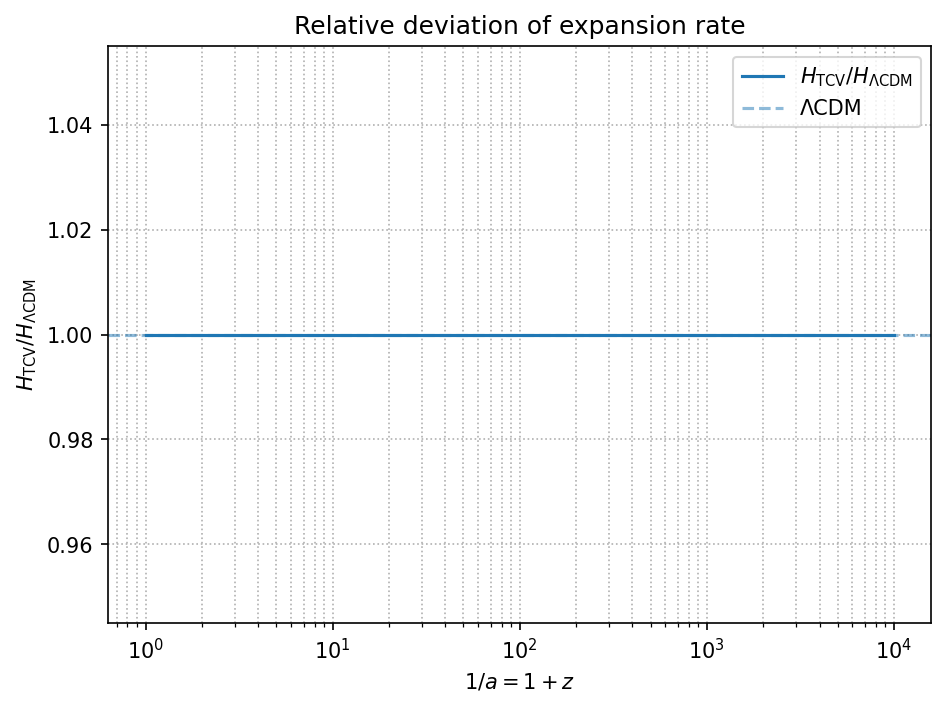
\includegraphics[width=0.7\textwidth]{../figs/tcv_background_H_ratio.png}
  \caption{
    Relative deviation of the TCV-$\phi$ background expansion rate with
    respect to a reference $\Lambda$CDM cosmology with identical
    $(H_0,\Omega_{\rm b} h^2,\Omega_{\rm c} h^2,\Omega_\Lambda,\Omega_{\rm r})$.
    The plot shows $\mathcal{R}_H(a) = H_{\rm TCV}(a)/H_{\Lambda{\rm CDM}}(a)$
    as a function of $1/a = 1+z$.
    By construction the two models share the same effective density parameters,
    so $\mathcal{R}_H(a)$ is numerically indistinguishable from unity over
    the range $10^{-4} \lesssim a \le 1$.
    This figure therefore acts mainly as a numerical sanity check of our
    CLASS interface and illustrates that, at the homogeneous level, the
    TCV-$\phi$ benchmark is exactly $\Lambda$CDM-like.
  }
  \label{fig:Hratio}
\end{figure}
% ----------------------------------------
\section{Linear matter power spectrum and fuzzy DM suppression}
\label{sec:Pk}
% ----------------------------------------

\subsection{Primordial spectrum and CLASS interface}

In the full TCV-$\phi$ programme, the primordial scalar power spectrum is intended to be computed from an explicit bounce dynamics and a modified Mukhanov--Sasaki equation with a cohesive pump field $z(\eta)$.
However, that calculation requires a separate and more complete treatment of the perturbations sector, which lies beyond the scope of Paper~I.
Here we simply adopt a standard nearly scale--invariant power law,
\begin{equation}
  \mathcal{P}_{\mathcal{R}}(k)
  = \As \left(\frac{k}{k_*}\right)^{\ns-1},
  \label{eq:primordial}
\end{equation}
with pivot $k_* = 0.05\,\mathrm{Mpc}^{-1}$, amplitude
\begin{equation}
  \As \simeq 2.1\times 10^{-9},
\end{equation}
and tilt $\ns\simeq 0.964$, close to the Planck 2018 value.
We set the tensor--to--scalar ratio to a negligible value, $r\approx 0$, consistent with both TCV--$\phi$ intuition and current upper bounds.

We then feed the effective parameter set~\eqref{eq:theta-tcv}, together with~\eqref{eq:primordial}, into the Boltzmann code CLASS via a small wrapper module \texttt{tcv\_boltzmann.py}.
The script \texttt{test\_tcv\_pk.py} calls CLASS to compute the linear matter power spectrum $P_{\rm cdm}(k,z)$ for a grid of wavenumbers $k$ at redshift $z=0$.
For numerical stability, we restrict ourselves to the range
\begin{equation}
  10^{-3} \lesssim k \lesssim 5~h\,\mathrm{Mpc}^{-1},
\end{equation}
well within the validity range of the CLASS computation for the chosen accuracy settings.

\subsection{Fuzzy DM transfer function}

The coherent ULDM field $\Phi_2$ behaves as pressureless matter at the background level, but its small--scale perturbations are subject to a scale--dependent suppression caused by its non--negligible de Broglie wavelength and quantum pressure.
Rather than implementing a full ULDM module in CLASS, we adopt in this first paper a phenomenological approach: we take the cold--dark--matter power spectrum $P_{\rm cdm}(k)$ delivered by CLASS and multiply it by a fuzzy--DM transfer function $T_{\rm F}(k)$,
\begin{equation}
  P_{\rm eff}(k) = T_{\rm F}^2(k)\,P_{\rm cdm}(k).
\end{equation}
We choose a simple two--parameter form,
\begin{equation}
  T_{\rm F}(k;k_J,n)
  = \frac{1}{\bigl[1+(k/k_J)^{2n}\bigr]},
  \label{eq:Tf-def}
\end{equation}
We stress that, at this stage, $T_{\rm F}(k)$ is \emph{not} derived from the full set of linear perturbation equations for the scalar field $\Phi_2$ in the TCV-$\phi$ EFT. Instead, it should be viewed as a simple two-parameter template inspired by the suppression found in dedicated ULDM studies such as Refs.~\cite{ULDM,Hui2017}. A realistic ULDM implementation in CLASS would predict a definite mapping
\begin{equation}
  (m_2,\Omega_{\Phi_2}) \longrightarrow (k_J,n),
\end{equation}
which we do not attempt to compute here. Our goal is simply to illustrate that, for plausible values of $(k_J,n)$, one can obtain a matter power spectrum that is indistinguishable from $\Lambda$CDM on large scales while exhibiting an ULDM-like damping on small scales.
where $k_J$ is an effective ``Jeans'' wavenumber and $n$ controls the sharpness of the transition.
For $k\ll k_J$, $T_{\rm F}\simeq 1$ and the power spectrum is indistinguishable from standard CDM.
For $k\gg k_J$, one has $T_{\rm F}\propto (k/k_J)^{-2n}$ and the power is strongly suppressed.

The mapping between $(m_2,\Omega_{\Phi_2})$ and $(k_J,n)$ in a realistic ULDM scenario is non--trivial and requires solving the full perturbation equations for the scalar.
For the purpose of Paper~I, we treat $(k_J,n)$ as effective parameters encoding the small--scale behaviour of the coherent field.
In our benchmark we adopt
\begin{equation}
  k_J \simeq 5~h\,\mathrm{Mpc}^{-1},
  \qquad
  n = 4,
\end{equation}
which yields a $\mathcal{O}(1)$ suppression of $P(k)$ around $k\sim k_J$ and a rapid fall--off at larger $k$.
For genuine ULDM models with $m_2 \sim 10^{-22}\,{\rm eV}$, dedicated calculations of the linear power spectrum typically find a half-mode scale $k_{1/2}$ of order a few $h\,{\rm Mpc}^{-1}$ (see e.g.\ Refs.~\cite{Hui2017,Marsh2016}).
Our choice $k_J \sim 5~h\,{\rm Mpc}^{-1}$ should therefore be viewed as representative of this ballpark, but we do not attempt to derive a precise mapping between $k_J$ and $m_2$ in this first paper.
Figure~\ref{fig:Pk_fuzzy} shows the resulting power spectrum at $z=0$ for three representative wavenumbers.\footnote{The accompanying script \texttt{test\_tcv\_pk.py} can be used to reproduce Fig.~\ref{fig:Pk_fuzzy} and to explore other benchmark choices of $(k_J,n)$.}

\begin{figure}[t]
  \centering
  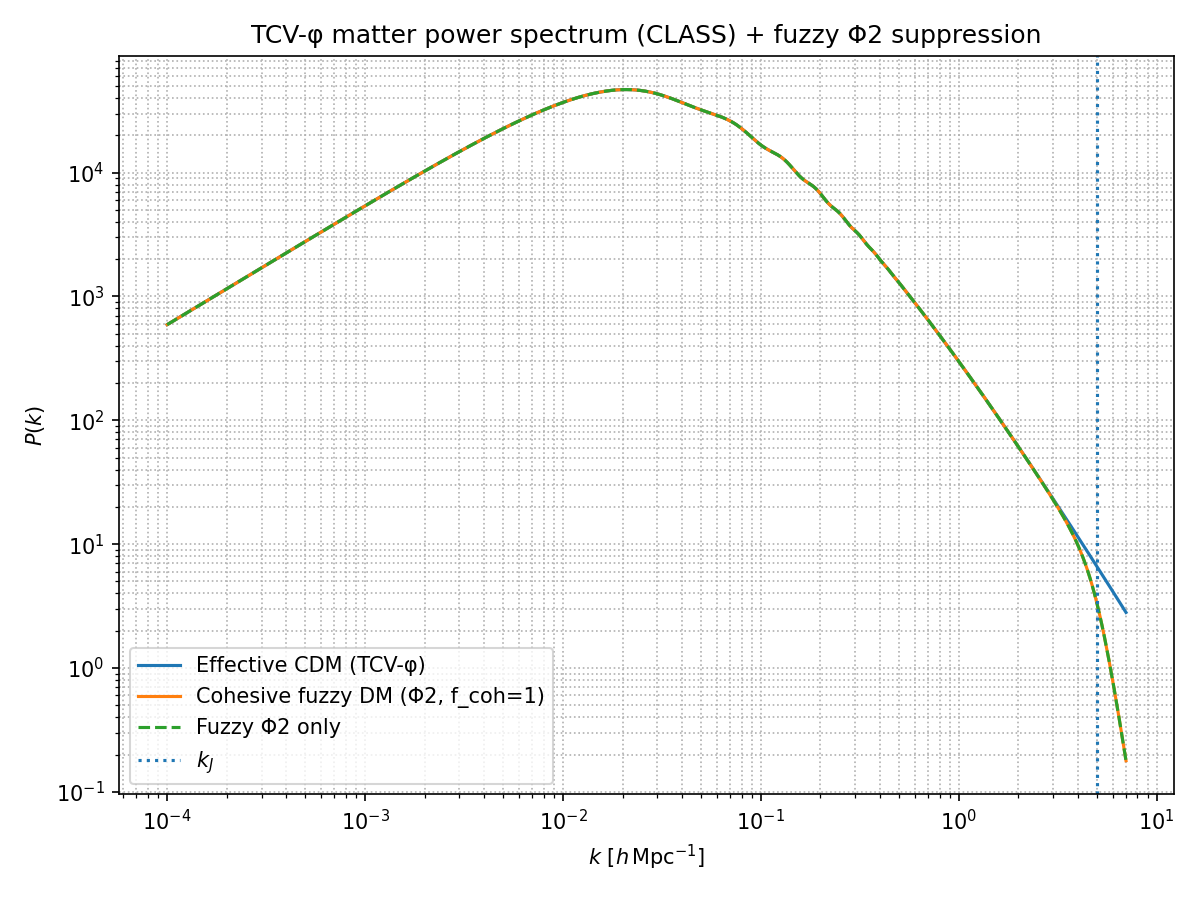
\includegraphics[width=0.65\textwidth]{../figs/tcvphi_pk_fuzzy.png}
  \caption{
    Schematic illustration of the TCV-$\phi$ linear matter power spectrum at $z=0$.
    The solid curve is the CLASS cold--dark--matter spectrum $P_{\rm cdm}(k)$ for the effective parameter set~\eqref{eq:theta-tcv}; the dashed curve shows the fuzzy--DM--modified spectrum $P_{\rm eff}(k)=T_{\rm F}^2(k)P_{\rm cdm}(k)$ with $k_J=5\,h\,\mathrm{Mpc}^{-1}$ and $n=4$.
    Within this phenomenological template, the resulting illustrative spectrum $P_{\rm eff}(k)$ coincides with $\Lambda$CDM on large scales and exhibits an ULDM--like suppression at small scales.
  }
  \label{fig:Pk_fuzzy}
\end{figure}

For this reason, Fig.~\ref{fig:Pk_fuzzy} should be understood purely as an illustrative template inspired by existing ULDM transfer functions, rather than as the prediction of the full set of linear perturbation equations for the cohesive vacuum EFT.

For our benchmark, we find numerically
\begin{align}
  k &= 0.1~h~\mathrm{Mpc}^{-1}:
  &
  P_{\rm cdm} &\sim 10^{4.2},
  &
  P_{\rm eff} &\sim 10^{4.2},
  \\
  k &= 1~h~\mathrm{Mpc}^{-1}:
  &
  P_{\rm cdm} &\sim 10^{2.5},
  &
  P_{\rm eff} &\sim 10^{2.5},
  \\
  k &= 5~h~\mathrm{Mpc}^{-1}:
  &
  P_{\rm cdm} &\sim 10^{0.8},
  &
  P_{\rm eff} &\sim 10^{0.5},
\end{align}
so that the suppression is negligible on quasi--linear scales and only becomes important on the smallest scales we probe, as expected from an ULDM--like behaviour.
A systematic comparison with current Lyman--$\alpha$ and dwarf--galaxy constraints on fuzzy dark matter is left for future work; here we simply demonstrate that the TCV-$\phi$ EFT can accommodate a phenomenologically reasonable ULDM--like suppression without spoiling the successful large--scale predictions of $\Lambda$CDM.

% ----------------------------------------
\section{Status of parameters and outlook}
\label{sec:discussion}
% ----------------------------------------

It is useful to summarize, at the end of this first TCV-$\phi$ paper, which quantities are taken as fundamental EFT parameters, which are derived at the cosmological level, and which remain phenomenological at this stage.

\begin{table}[t]
  \centering
  \begin{tabular}{lcc}
    \hline\hline
    Parameter & Meaning & Benchmark value \\
    \hline
    $m_1$       & structural mass scale & $10^{11}~\mathrm{GeV}$ \\
    $\Phi_0$    & minimum of $V_1$      & $10^{11}~\mathrm{GeV}$ \\
    $\lambda_1$ & quartic self-coupling & $10^{-2}$ \\
    $\xi_0$     & non-minimal coupling  & $0.1$ \\
    $m_2$       & ULDM mass             & $10^{-22}~\mathrm{eV}$ \\
    $\Phi_{2,0}$& misalignment amplitude& $1.1\times 10^{17}~\mathrm{GeV}$ \\
    $k_J$       & fuzzy--DM scale       & $5~h\,\mathrm{Mpc}^{-1}$ \\
    $n$         & sharpness exponent    & $4$ \\
    \hline\hline
  \end{tabular}
  \caption{Benchmark parameter set used throughout this paper.}
  \label{tab:benchmarks}
\end{table}

\paragraph*{Microscopic EFT parameters.}
The core TCV-$\phi$ EFT is characterized by
\begin{equation}
  \{m_1,\Phi_0,\lambda_1,\xi_0,m_2,\rho_{\rm vac},\Mpl\},
\end{equation}
with $m_1\sim\Phi_0\sim 10^{11}\,\mathrm{GeV}$, $\lambda_1\ll 1$, $\xi_0\ll1$, and $m_2\simeq 10^{-22}\,\mathrm{eV}$ in the benchmark.
In future work these parameters will be connected to a more detailed cohesive microphysics (cluster picture, quantum corrections, etc.).
In Paper~I we simply require that they lead to a stable minimum $V_1(\Phi_0)$, a small effective cosmological constant and a ULDM--like mass $m_2$.

\paragraph*{Cosmological parameters.}
The homogeneous cosmology is then specified by
\begin{equation}
  H_0,\ \omega_{\rm b},\ \omega_{\rm dm},\ \As,\ \ns,\ r,
\end{equation}
as in standard $\Lambda$CDM, together with a misalignment amplitude $\Phi_{2,0}$ for the coherent field.
In this first paper we choose these parameters to be close to Planck--2018 and to match the observed dark matter abundance via the misalignment estimate~\eqref{eq:misalignment}.
We do not yet attempt to derive $\Phi_{2,0}$ from $\Phi_1$ or to connect $(\As,\ns)$ to the bounce dynamics; that is the purpose of later TCV-$\phi$ papers focused on the primordial sector.

\paragraph*{Fuzzy--DM phenomenology.}
The small--scale suppression of $P(k)$ induced by $\Phi_2$ is captured in this paper by a simple transfer function~\eqref{eq:Tf-def} with parameters $(k_J,n)$.
A realistic ULDM model would predict a mapping
\begin{equation}
  (m_2,\Omega_{\Phi_2}) \longrightarrow (k_J,n).
\end{equation}
In Paper~I, however, we treat $(k_J,n)$ as an effective parametrization of the fuzzy--DM effect, chosen to be consistent with the benchmark $m_2$ and to leave large scales essentially unaffected.

\medskip

In summary, Paper~I establishes that:
\begin{enumerate}[label=(\roman*),leftmargin=1.5em]
  \item A minimal cohesive--vacuum EFT with two scalar fields $\Phi_1$ and $\Phi_2$ can reproduce a $\Lambda$CDM--like background cosmology for reasonable values of its microscopic parameters;
  \item The coherent field $\Phi_2$ naturally behaves as an ULDM component at late times, with misalignment amplitude $\Phi_{2,0}$ chosen to match the observed dark matter abundance;
  \item Interfacing the TCV-$\phi$ EFT with CLASS and applying a simple fuzzy--DM transfer function yields, within this phenomenological template, an illustrative spectrum $P_{\rm eff}(k)$ that coincides with $\Lambda$CDM on large scales and exhibits an ULDM--like suppression at small scales.
\end{enumerate}
From a phenomenological point of view, the TCV-$\phi$ framework can therefore be viewed as a consistent reinterpretation of standard $\Lambda$CDM+ULDM cosmology in terms of a cohesive vacuum EFT.
We have not attempted, in this first step, to go beyond this standard phenomenology or to provide new observational signatures. Instead, the present work should be viewed as a definition and basic sanity check of the cohesive--vacuum EFT, paving the way for subsequent papers where the same Lagrangian will be used to address the primordial sector (bounce and perturbations), baryogenesis and strong-field objects.

\appendix

\section{Non--minimal coupling and variation of $M_{\rm eff}$}
\label{app:Meff}

For completeness, we briefly justify the neglect of the non--minimal terms proportional to derivatives of $M_{\rm eff}(\Phi_1)$ in the background equations used in this paper. Starting from Eq.~\eqref{eq:Meff}, the effective Planck mass reads
\begin{equation}
  M_{\rm eff}^2(\Phi_1) = M_{\rm Pl}^2\left(1 + \xi_0 \frac{\Phi_1^2}{M_{\rm Pl}^2}\right).
\end{equation}
A change in $\Phi_1$ between two epochs translates into a variation of the effective Newton constant,
\begin{equation}
  \frac{\Delta G}{G}
  \simeq - \frac{\Delta M_{\rm eff}^2}{M_{\rm eff}^2}
  \simeq - 2\,\xi_0\,\frac{\Phi_0\,\Delta\Phi_1}{M_{\rm Pl}^2},
\end{equation}
where we have expanded around the minimum $\Phi_1 \simeq \Phi_0$ and assumed $|\Delta\Phi_1|\ll \Phi_0$. In our benchmark, $m_1 \sim \Phi_0 \sim 10^{11}~{\rm GeV}$ and $\xi_0 \sim 0.1$, so that the relaxation time scale of the structural field is of order $m_1^{-1}$, many orders of magnitude shorter than the Hubble time at any cosmological epoch of interest (BBN, recombination, late times). As a result, $\Phi_1$ settles to its minimum long before BBN and remains extremely close to $\Phi_0$ afterwards, with $|\Delta\Phi_1|/\Phi_0 \ll 10^{-8}$ over the entire observable cosmological history.

This implies
\begin{equation}
  \left|\frac{\Delta G}{G}\right|
  \lesssim 2\,\xi_0\,\frac{\Phi_0^2}{M_{\rm Pl}^2}
  \sim 2\times 0.1 \left(\frac{10^{11}}{2.4\times 10^{18}}\right)^2
  \sim 10^{-16}.
\end{equation}
Given $m_1 \sim 10^{11}~{\rm GeV}$, the relaxation time of the structural field is of order
$\tau_{\rm rel} \sim m_1^{-1} \sim 10^{-35}\,{\rm s}$, i.e.\ many orders of magnitude shorter
than the Hubble time at reheating or during Big Bang nucleosynthesis (BBN).
It is therefore reasonable to assume that $\Phi_1$ settles to its minimum $\Phi_0$ well before BBN and remains extremely close to it afterwards.
Typical bounds on the variation of Newton's constant from BBN, CMB and local tests are at the level $|\Delta G/G| \lesssim 10^{-2}$ or $|\dot G/G|\lesssim 10^{-12}\,{\rm yr}^{-1}$ (see e.g.\ the review~\cite{Uzan2011}), so our estimate $|\Delta G/G|\sim 10^{-16}$ is safely many orders of magnitude below current limits.
The same small parameter suppresses the time derivatives $\dot M_{\rm eff}$ and $\ddot M_{\rm eff}$ in the modified Friedmann and Klein--Gordon equations.

% ----------------------------------------
%\section*{Acknowledgements}
% ----------------------------------------

%The author thanks [names to be added] for numerous discussions and constructive feedback on earlier drafts of the TCV-$\phi$ programme.

% ----------------------------------------
% Bibliography (skeleton; to be completed)
% ----------------------------------------

\begin{thebibliography}{99}

\bibitem{Planck2018}
N.~Aghanim \textit{et al.} [Planck Collaboration],
``Planck 2018 results. VI. Cosmological parameters,''
Astron.\ Astrophys.\ \textbf{641}, A6 (2020)
[arXiv:1807.06209].

\bibitem{CLASS}
D.~Blas, J.~Lesgourgues and T.~Tram,
``The Cosmic Linear Anisotropy Solving System (CLASS). Part II: Approximation schemes,''
JCAP \textbf{07}, 034 (2011)
[arXiv:1104.2933].

\bibitem{ULDM}
W.~Hu, R.~Barkana and A.~Gruzinov,
``Fuzzy Cold Dark Matter: The wave properties of ultralight particles,''
Phys.\ Rev.\ Lett.\ \textbf{85}, 1158 (2000)
[arXiv:astro-ph/0003365].

\bibitem{Hui2017}
L.~Hui, J.~P.~Ostriker, S.~Tremaine and E.~Witten,
``Ultralight scalars as cosmological dark matter,''
Phys.\ Rev.\ D \textbf{95}, 043541 (2017)
[arXiv:1610.08297].

\bibitem{Marsh2016}
D.~J.~E.~Marsh,
``Axion cosmology,''
Phys.\ Rept.\ \textbf{643}, 1-79 (2016)
[arXiv:1510.07633].

\bibitem{Uzan2011}
J.~P.~Uzan,
``Varying constants, gravitation and cosmology,''
Living Rev.\ Relativ.\ \textbf{14}, 2 (2011).

\bibitem{Clifton2012}
T.~Clifton, P.~G.~Ferreira, A.~Padilla and C.~Skordis,
``Modified gravity and cosmology,''
Phys.\ Rept.\ \textbf{513}, 1-189 (2012)
[arXiv:1106.2476].

\bibitem{Schive2014}
H.~Y.~Schive, T.~Chiueh and T.~Broadhurst,
``Cosmic structure as the quantum interference of a coherent dark wave,''
Nature Phys.\ \textbf{10}, 496--499 (2014)
[arXiv:1406.6586].

\end{thebibliography}

\end{document}
